\documentclass{zah}

\title{Návrh systému evidencie plynových fliaš}
\author{Oliver Laštík, Šimon Strieška, Jozef Špirka, Adam Zahradník}

\begin{document}
\maketitle

\tableofcontents
\cleardoublepage

\section{Špecifikácia vonkajších interfejsov}

Systém beží na webovom serveri, ku ktorému používateľ pristupuje cez webový prehliadač. Webový server poskytuje užívateľovi prístup k funkcionalitám systému prostredníctvom HTTPS protokolu. Systém uchováva informácie o plynových fľašiach a používateľoch v databáze. Na komunikáciu s databázou využíva framework Django. Databázové dotazy sú zasielané na server cez SQL protokol. Systém komunikuje s používateľom prostredníctvom grafického rozhrania (GUI) vo webovom prehliadači. GUI poskytuje užívateľovi možnosť nahrávať fotografie manometra, zobrazovať, pridávať, mazať, upravovať a exportovať údaje o plynových fľašiach. Pri pokuse o detekciu manometra systém komunikuje s kamerou daného zariadenia. Pri prvom pokuse o detekciu manometra si systém vyžiada povolenie od používateľa na používanie kamery. Interakcia s kamerou prebieha cez natívne API pre kamery v danom zariadení.

\section{Dátový model}
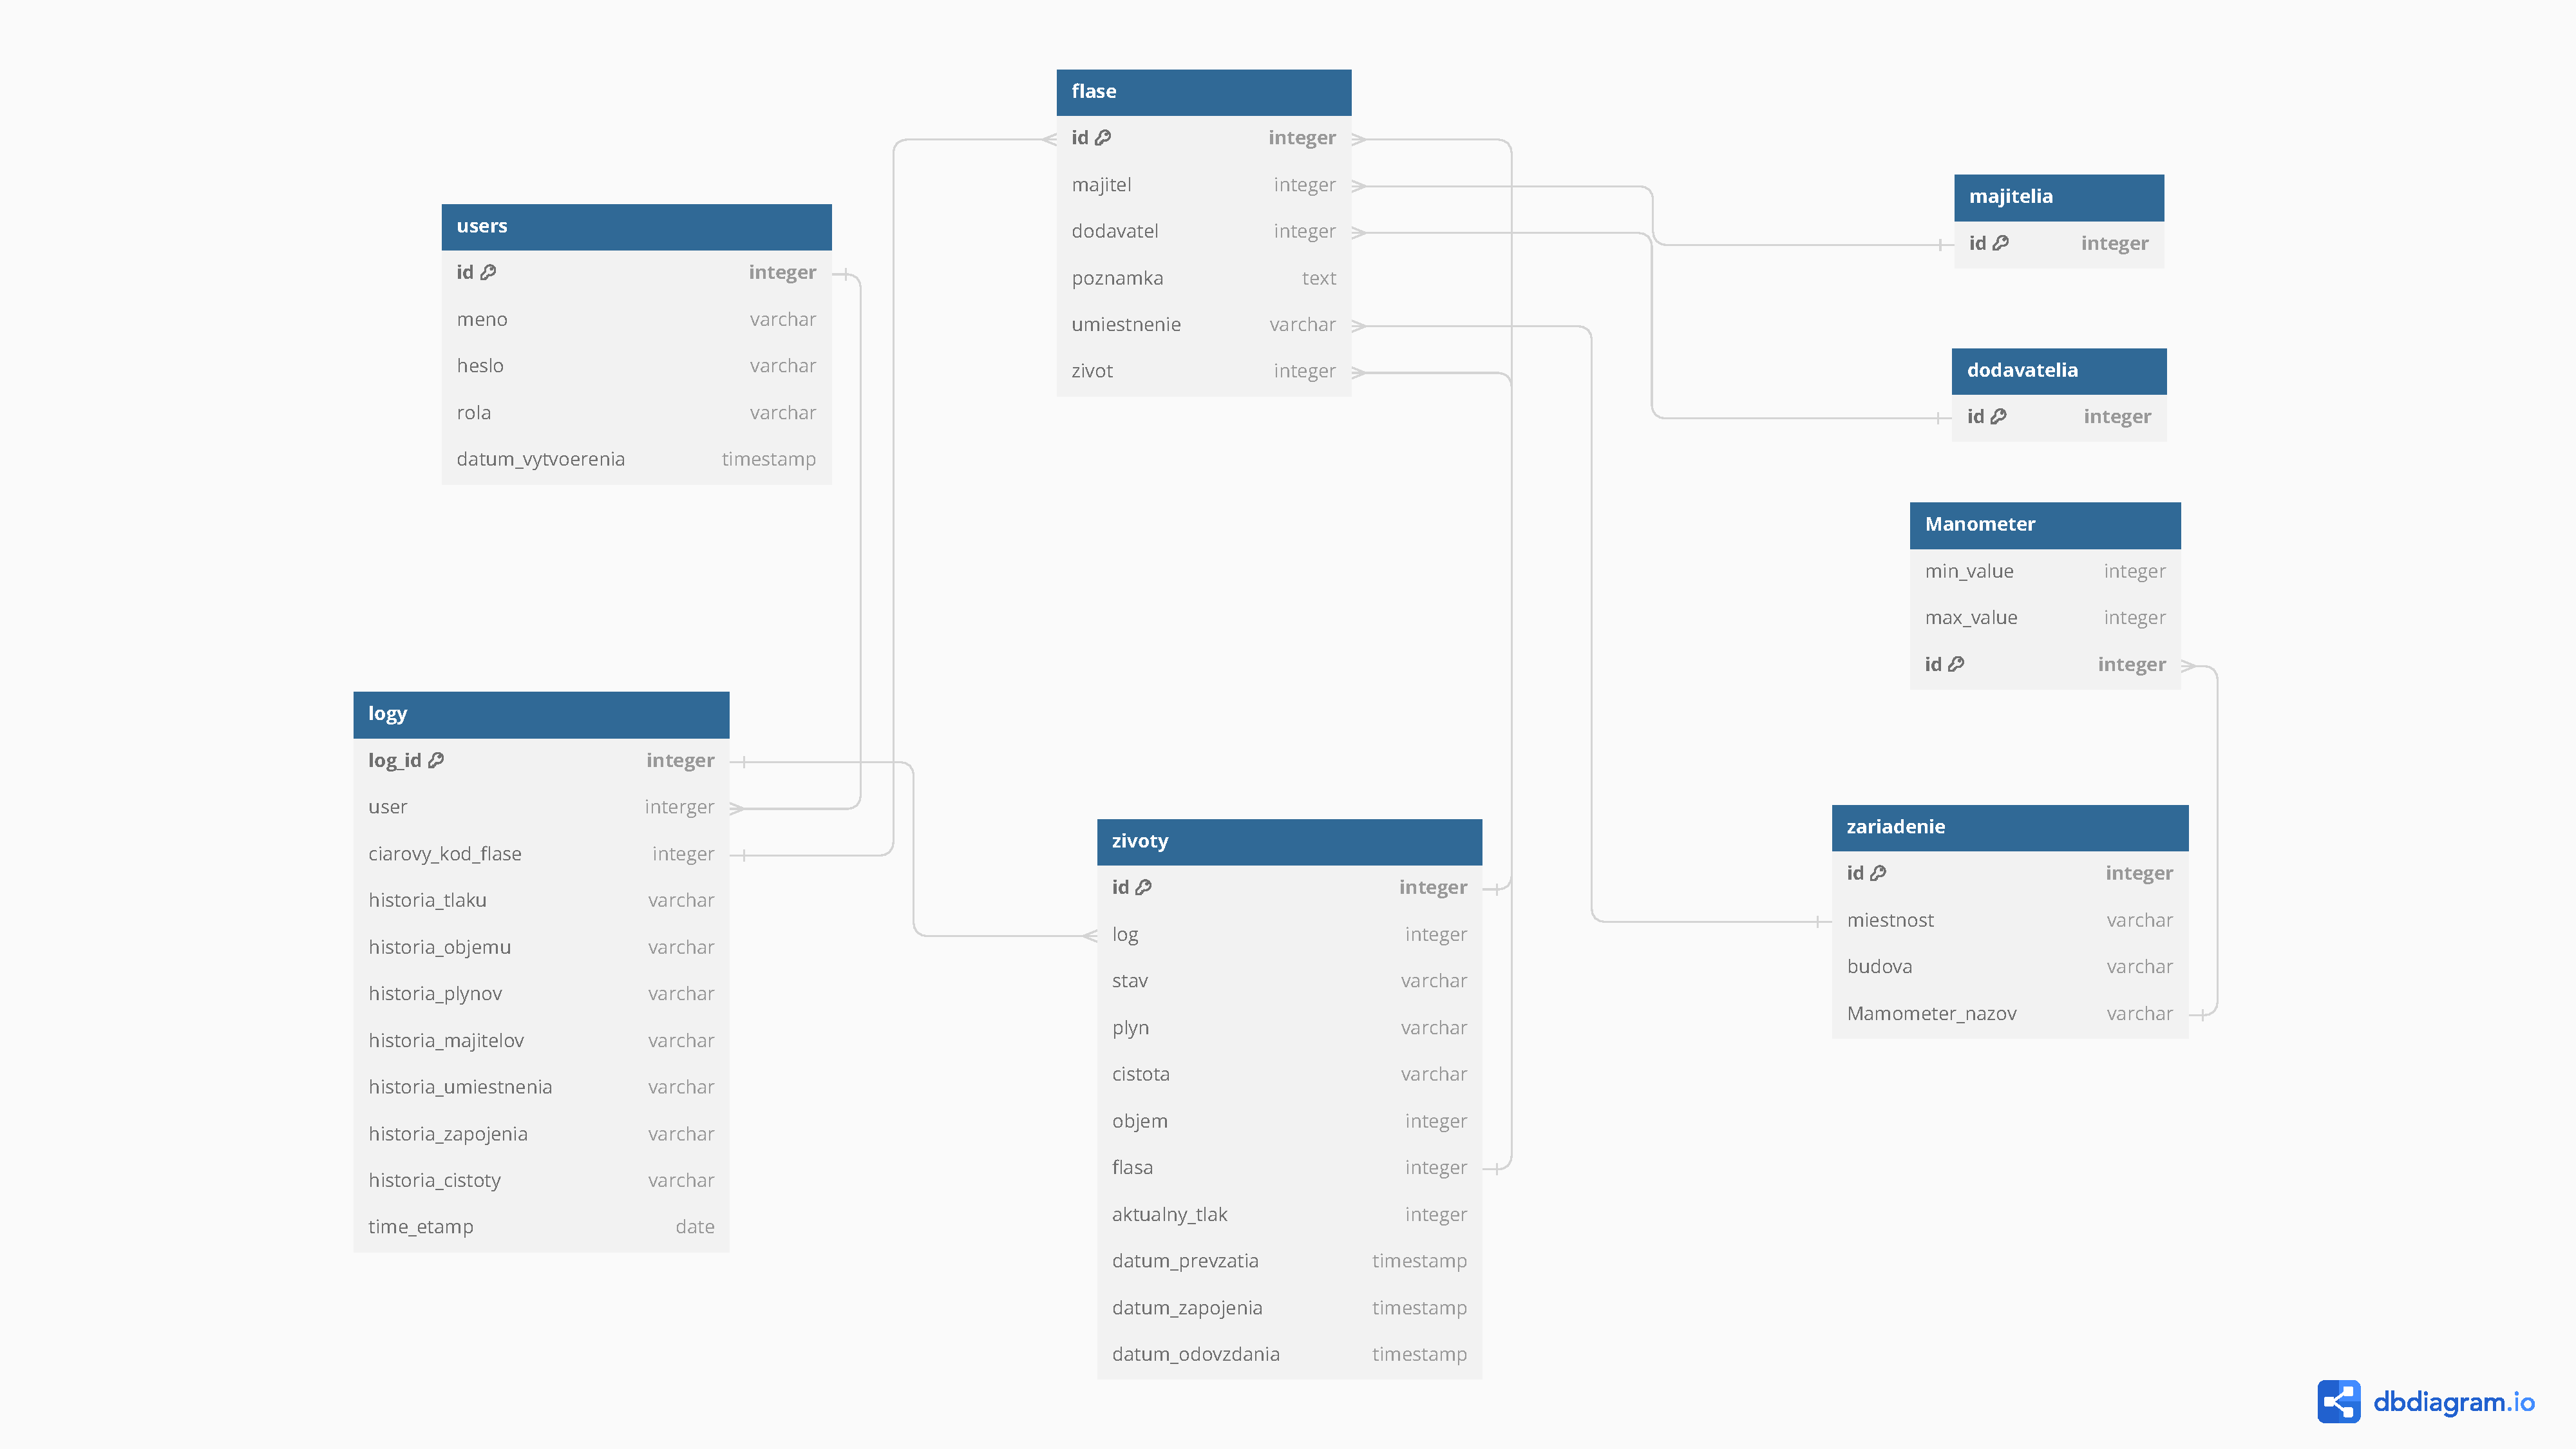
\includegraphics[width=\textwidth]{navrh-assets/db}

Databáza sa skladá z viacerých tabuliek, ktoré sú navzájom prepojené cez cudzie kľúče. Hlavné tabuľky zahŕňajú:

\begin{itemize}
    \item \textbf{flase\_app\_user}: Obsahuje informácie o používateľoch systému vrátane ich rolí a autentifikačných údajov.
    \item \textbf{flase\_app\_cylinder}: Uchováva záznamy o jednotlivých fľašiach, ich umiestnení, vlastníkoch a životných cykloch.
    \item \textbf{flase\_app\_cylinderlife}: Zaznamenáva rôzne stavy fľaši, vrátane údajov o tlaku, plyne a objeme.
    \item \textbf{flase\_app\_cylinderchange}: Uchováva logy súvisiace s operáciami a udalosťami týkajúcimi sa fľaši.
    \item \textbf{flase\_app\_supplier}, \textbf{flase\_app\_gas}, \textbf{flase\_app\_owner}, \textbf{flase\_app\_location}, \textbf{flase\_app\_workplace},\textbf{flase\_app\_building}: Tieto tabuľky poskytujú dodatočné informácie o dodávateľoch, vlastníkoch, plynoch, umiestneniach, pracovnom prostredi a budove spojených s fľašami.
\end{itemize}

Každá tabuľka je navrhnutá s cieľom optimalizovať ukladanie a prístup k dátam potrebným pre správu a sledovanie fľaši a súvisiacich aktivít.

\subsection{Formáty súborov}
\subsubsection{Konfigurácia systému}

Systém sa konfiguruje pomocou tzv. premenné prostredia (environment variables).
Tento systém je vhodný, ak je aplikácia nasadzovaná do kontajnerizovaného prostredia,
alebo je spravovaný supervisorom, ako napríklad SystemD, ktorý jej vie tieto premenné poskytnúť.
Pre jednoduchšie nasadzovanie je však možné použiť súbor \texttt{.env}, vo formáte: \texttt{VARIABLE=value}.

Systém podporuje tieto premenné:

\begin{itemize}
	\item \texttt{SECRET\_KEY} náhodný string používaný na šifrovanie session dát
	\item \texttt{DEBUG} boolean (predvolene False), ktorý určuje, či Django vypisuje všetky chyby a zapína debugger
	\item \texttt{ALLOWED\_HOSTS} čiarkou oddelený zoznam domén, na ktorých je náš systém dostupný
	\item \texttt{DATABASE\_URL} adresa databázy, vrátane prístupových údajov (ak treba), pre celý syntax pozri \href{https://django-environ.readthedocs.io/en/latest/types.html#environ-env-db-url}{dokumentáciu}, predvolene používa SQLite3 databázu \texttt{db.sqlite3}
	\item \texttt{EMAIL\_FROM} a \texttt{EMAIL\_URL} nastavuje odosielanie emailov. Predvolene sa maily píšu na štandardný výstup, nastavenie SMTP a iných spôsobov nájdete \href{https://django-environ.readthedocs.io/en/latest/types.html#environ-env-email-url}{v dokumentácií}
\end{itemize}

\subsubsection{CSV export}

Systém poskytuje používateľom možnosť vyexportovať aktuálny stav skladu.
Výsledok tejto operácie je súbor formátu CSV (hodnoty oddelené čiarkou) s nasledujúcimi stĺpcami:
barcode, gas, volume, pressure, pressure\_date, location, is\_connected, owner, supplier, note.

\subsection{Stavový diagram}
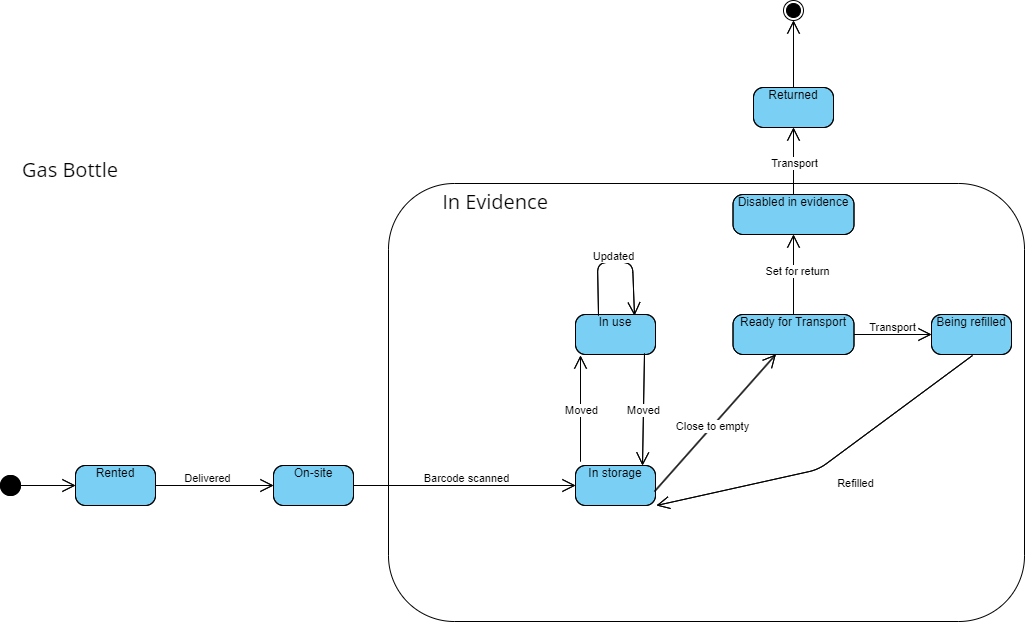
\includegraphics[width=\textwidth]{navrh-assets/state}

Stavový diagram modeluje správanie plynovej fľaše v systéme. Fľaša je v počiatočnom stave Rented, keď je prenajatá.
Po prenájme je fľaša s plynom doručená na fakultu, kde nadobúda stav On-site. Oscanovaním čiarového kódu je 
flaša pridaná do systému a získava stav In Storage, kde je uskladnená, ale práve sa nepoužíva. Stav flaše sa
môže opakovane meniť medzi In Storage a In Use, poďľa toho či je využivaná alebo nie. Flaša, ktorá je skoro prázdna
je presunutá zo skladu a pripravená na prepravu, nadobúda stav Ready for Transport. Flaša je v stave Being refilled,
ak je vybraná pre naplnenie, po naplnení je vrátená do skladu a nadobúda stav In Storage. Ak je fľaša vybraná na navrátenie
majiteľovi, tak je označená v systéme ako neaktívna a získava stav Disabled in evidence. Po transporte majiteľovi nadobúda
koncový stav Returned.

\section{Návrh používateľského rozhrania}

\subsection{Prihlasovacia obrazovka}
\begin{center}
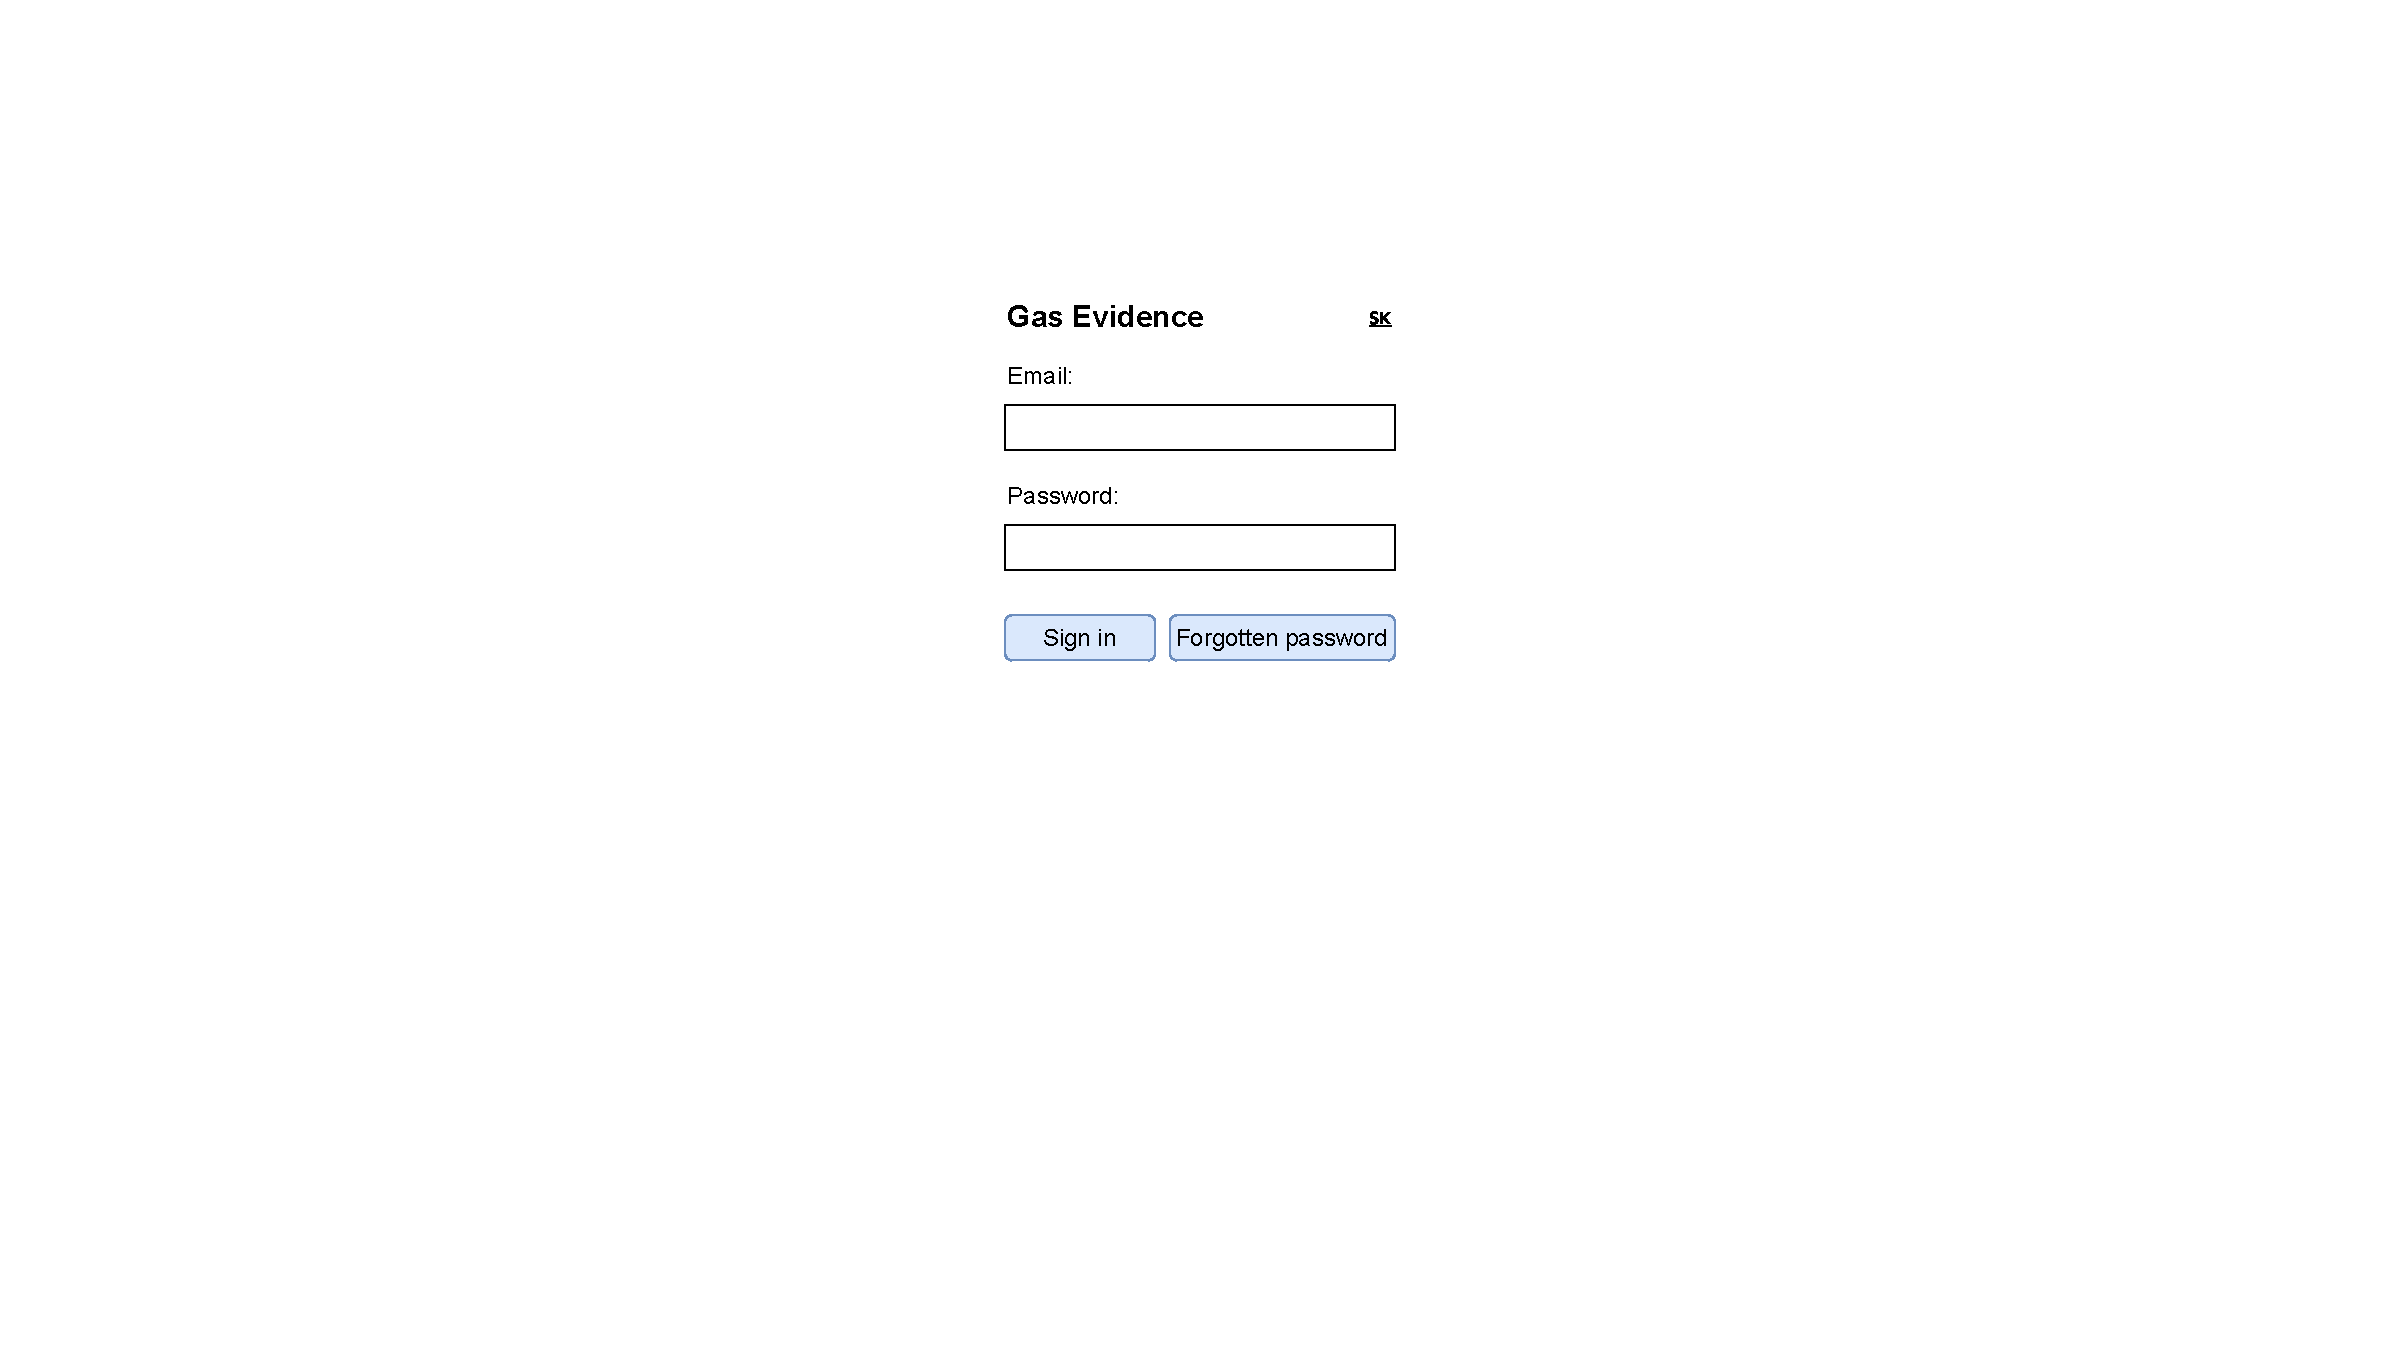
\includegraphics[width=.7\textwidth,page=1]{navrh-assets/ui}
\end{center}

\subsection{Navigačné menu}
\begin{center}
\includegraphics[width=.7\textwidth,page=2]{navrh-assets/ui}
\end{center}

\subsection{Zoznam fliaš}
\begin{center}
\includegraphics[width=.7\textwidth,page=3]{navrh-assets/ui}
\end{center}

Na mobilnom zariadení sa miesto tabuľky zobrazí vertikálny zoznam.

\subsection{Detail fľaše}
\begin{center}
\includegraphics[width=.7\textwidth,page=4]{navrh-assets/ui}
\end{center}

\subsection{Úprava fľaše}
\begin{center}
\includegraphics[width=.7\textwidth,page=5]{navrh-assets/ui}
\end{center}

\subsection{Pridanie fľaše}
\begin{center}
\includegraphics[width=.7\textwidth,page=6]{navrh-assets/ui}
\end{center}


\subsection{Zoznam dodávateľov}
\begin{center}
\includegraphics[width=.7\textwidth,page=7]{navrh-assets/ui}
\end{center}
Analogicky pre majiteľov a plyny.

\subsection{Pridanie/úprava dodávateľov}
\begin{center}
\includegraphics[width=.7\textwidth,page=8]{navrh-assets/ui}
\end{center}
Analogicky pre majiteľov a plyny.

\subsection{Zoznam používateľov}
\begin{center}
\includegraphics[width=.7\textwidth,page=9]{navrh-assets/ui}
\end{center}

\subsection{Pridávanie/úprava používateľov}
\begin{center}
\includegraphics[width=.7\textwidth,page=10]{navrh-assets/ui}
\end{center}

\subsection{Fotenie manometra}
\begin{center}
\includegraphics[width=.7\textwidth,page=11]{navrh-assets/ui}
\end{center}
Na pravo výsledok merania, dá sa ručne upraviť v prípade zlej detekcie.

\section{Návrh implementácie}

\subsection{Component diagram}
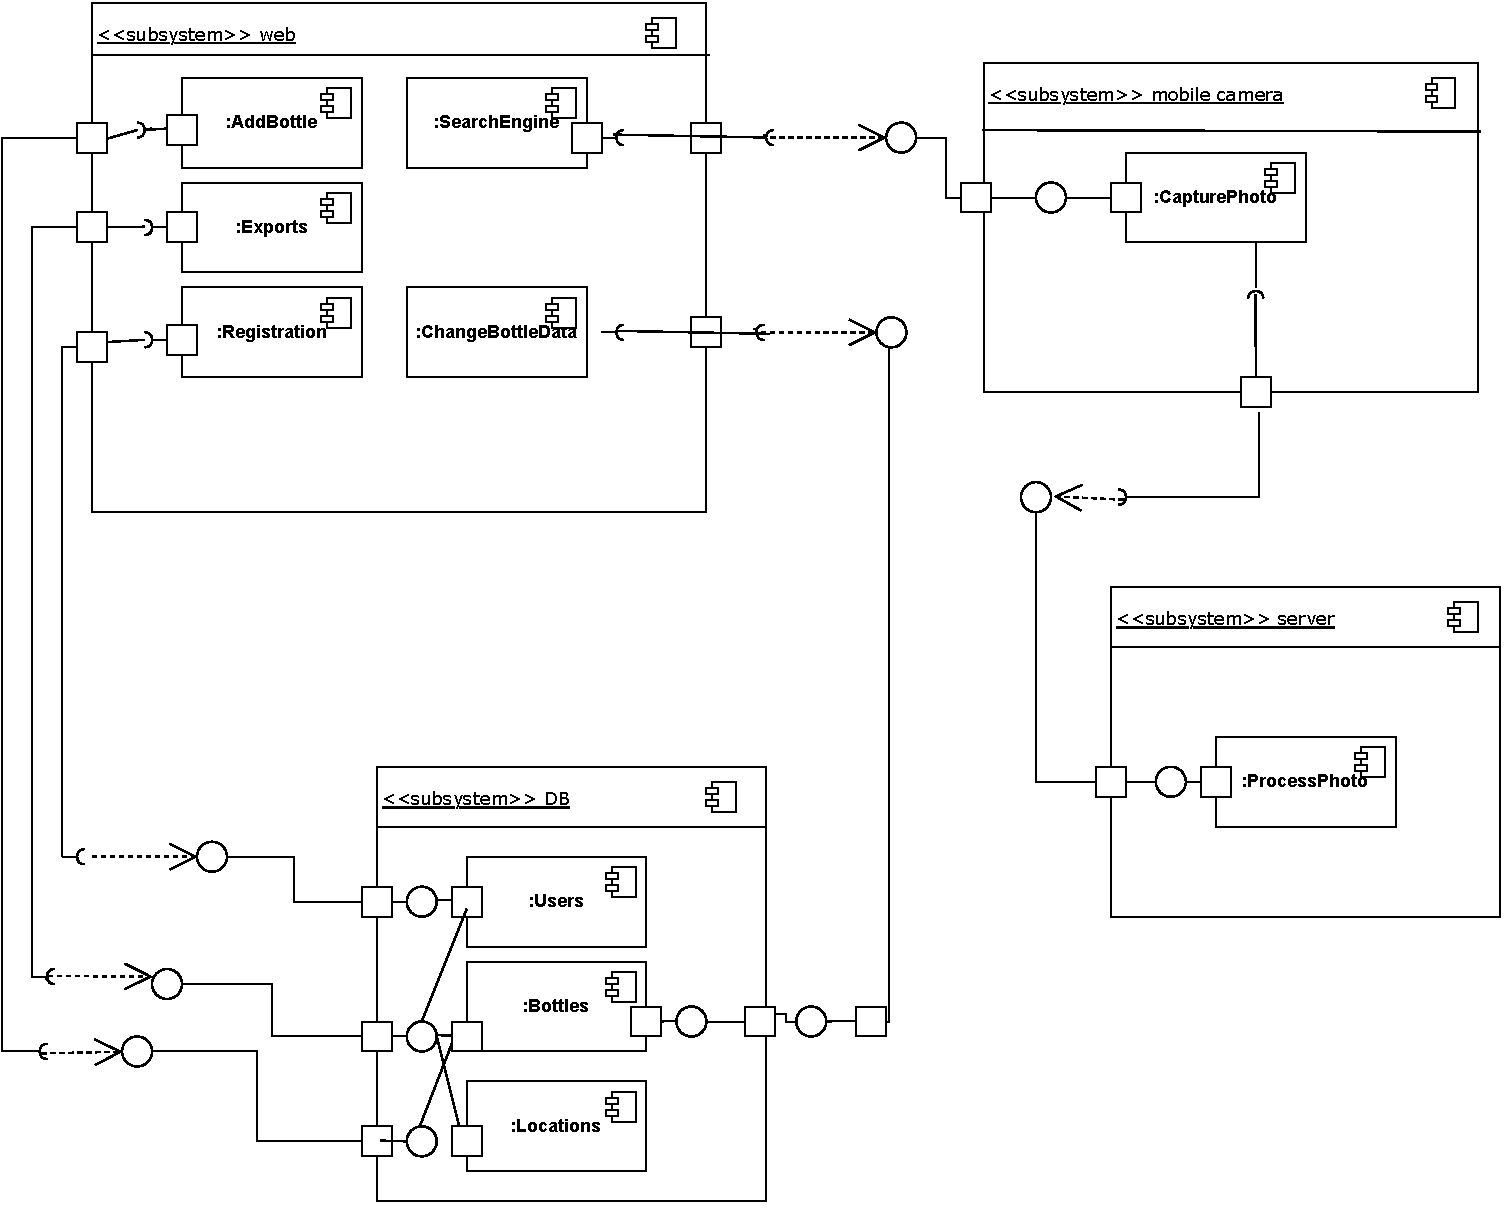
\includegraphics[width=\textwidth]{navrh-assets/component}

Vo webovom prehliadači má používateľ dostupné komponenty ako zobrazovanie, pridávanie,
filtrovanie, vyhľadávanie, menenie dát fľaše, sťahovanie fľaší do excelu. Všetky
komponenety komunikujú s databázou a výsledky sa zobrazia na webe. Pri pridávaní,
vyhľadávaní a zmene dát flaše je možné požiadať telefón o mobilnú kameru.
Po odfotení fotografie sa fotografia spracuje buď vo webovom prehliadači, alebo mobil
komunikuje so serverom, kde sa fotografia spracuje. Po spracovaní sa opäť komunikuje
s databázou a výsledky sa zobrazia na webe.

\section{Deployment}
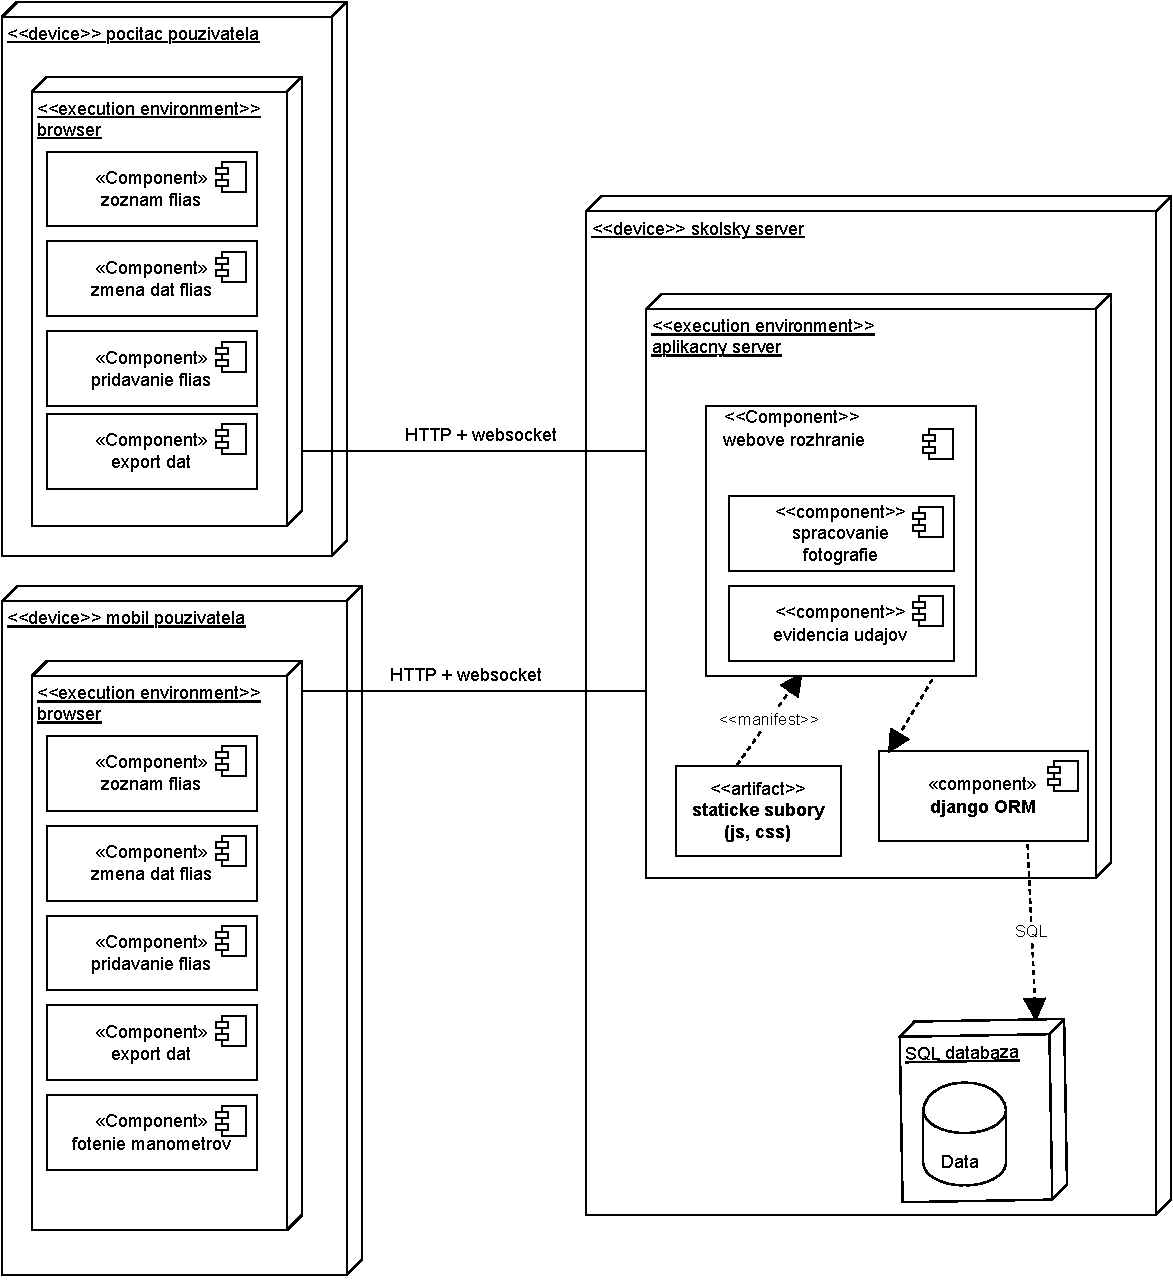
\includegraphics[width=\textwidth]{navrh-assets/deployment}

Keďže systém vzniká ako webová aplikácia, bude sa nasadzovať na aplikačný server.
Tento aplikačný server, v našom prípade \textit{gunicorn} alebo \textit{mod\_wsgi} spúšťa samotnú
Django aplikáciu, ktorá obsluhuje požiadavky. Pred týmto aplikačným serverom sa môže nachádzať aj
reverzná proxy v podobe webového servera \textit{Apache} alebo \textit{nginx}.

Aplikácia sa bude nasadzovať primárne na server s operačným systémom Linux, avšak vzhľadom na
medzi-platformovú kompatibilitu jazyka Python by nemal byť problém systém nasadiť aj na systéme Windows.

\section{Použité technológie}

Pri realizácií projektu sme sa rozhodli použiť nasledujúce webové technológie:

\begin{itemize}
\item Python sme si vybrali ako primárny jazyk pre jeho jednoduchosť,
	vysokú medzi-platformovú kompatibilitu a prítomnosť OpenCV knižnice.
\item Django je jeden z populárnych webových frameworkov pre Python. 
	Poskytuje nám kvalitné, bezpečné jadro a flexibilný 
	systém na prácu s databázou. Django je dlhodobo veľmi stabilné,
	preto aj neskoršie úpravy systému nebudú sprevádzané problémami.
\item Na vývoj webového rozhrania sme použili štandardné webové technológie
	HTML, CSS, JS spolu s CSS frameworkom Bootstrap, ktorý nám ponúka ucelený
	design systému.
\item Na vykreslovanie grafov využijeme knižnicu Chart.js a na skenovanie čiarových
	kódov mobilom využijeme html5-qrcode. Knižnica sa síce nazýva qrcode, ale podporuje
	aj klasické 1D kódy. Vybrali sme si ju primárne kvôli podpore hardvérovej akcelerácií
	skenovania kódov.
\item Pri výbere databázového systému sme zvolili SQLite3. Najmä pre jej jednoduché
	nasadzovanie do prevádzky a jednoduchú správu (zálohovanie a pod.). Keby sa v budúcnosti
	preukázala SQLite3 ako nedostatočná, vďaka využitiu Django ORM systému je možné databázu
	jednoducho vymeniť za Postgres, resp. MySQL.
\item Na automatické rozoznávanie tlaku z manometrov využijeme knižnice OpenCV na 
	spracovávanie obrazových dát a NumPy na potrebné matematické výpočty.
	\href{https://github.com/TIS2023-FMFI/evidencia-flias/tree/Manometre-demo/Demo}{Túto kombináciu sme testovali tu.}
\end{itemize}

\section{Plán implementácie}

\begin{enumerate}
	\item Prihlasovanie používateľov
	\item Zoznam a správa majiteľov
	\item Zoznam a správa dodávateľov
	\item Zoznam a správa plynov
	\item Zoznam a správa používateľov
	\item Zoznam fliaš
	\item Vyhľadávanie fliaš
	\item Filtrovanie fliaš
	\item Príjem nových fliaš
	\item Menenie parametrov fľaše
	\item Zobrazovanie histórie fliaš
	\item Manuálne zadávanie tlaku
	\item Export dát
	\item Automatické rozoznávanie tlaku
\end{enumerate}

\end{document}
